\documentclass{beamer}

\usetheme{simple}

\usepackage{lmodern}
\usepackage{tabularx}
\usepackage{amssymb}% http://ctan.org/pkg/amssymb
\usepackage{pifont}

% short cut for tick and cross commands
\newcommand{\yes}{\checkmark}
\newcommand{\no}{\hspace{1pt}\ding{55}}

\usepackage[scale=2]{ccicons}

%\setwatermark{\includegraphics[height=1.3cm]{img/watermark.jpg}}

\newcommand\pro{\item[\textbf{+}]}
\newcommand\con{\item[\textbf{--}]}

\title{Music synthesis with FPGAs \\and open-source tools}
\subtitle{}
\author{\texttt{github.com/schnommus/eurorack-pmod}}
\institute{Sebastian Holzapfel}
\date{}
\titlegraphic{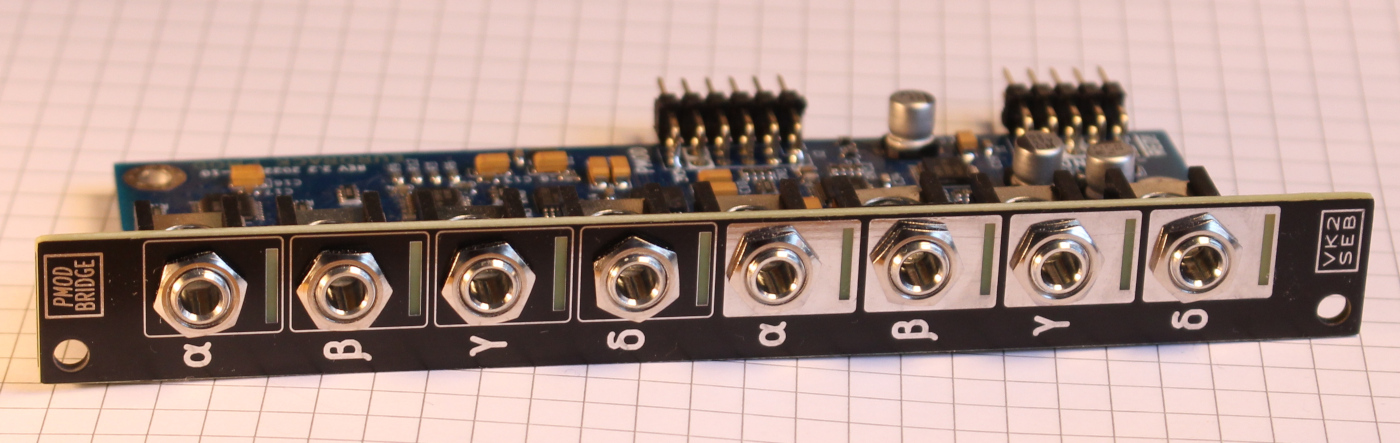
\includegraphics[height=3cm]{img/eurorack-pmod.jpg}}

\begin{document}

\maketitle

\setwatermark{}

% OUTLINE

% why eurorack?
% why eurorack-pmod?
% evolution, how it works
% (no hardware!) sim vcv & sim testbenches
% (interest?) revision 3 and manufacturing
% stay creative

% What is Eurorack?
% Simple Eurorack system (emph. DC/CV + Audio same jacks, requirements)
% Existing FPGA-based modules (v short)
% & existing development platforms (v short)

% What is EURORACK-PMOD
% Connect to any FPGA development board like such
% Lets you write simple Verilog and explore sound
% Examples in the repository (etc...)
% Specific example

% How does this work?

% INTERESTING THINGS
% HARDWARE
% - AK4619
% - Hardware evolution
% - DC coupling & calibration
%   - Misused. Price point. Fortunately outputs are DC coupled (register allows misuse)!
% - Latency
% - Light bleed mechanism
% - Revision 3
% GATEWARE
% - Simple example cores / demo
% SIMULATION
% - VCVRack demo
% - Test benches

% CUSTOM PICS/VIDS NEEDED
% - My eurorack system
% - ICEbreaker and connected to ICEbreaker
% - Latency on scope
% - Prototypes r1 2 and 3 (next to each other?)
% - VCVrack screen capture
% - 2x video demos

\begin{frame}{Outline}

    \begin{itemize}
        \item Item A
        \item Preliminary work \& demo
    \end{itemize}

    \begin{block}{Mechanisms for:}
        \begin{itemize}
            \item FPGAs
            \item Synthesis
        \end{itemize}
    \end{block}

\end{frame}


\end{document}
